\documentclass[pl]{minipw} % wszystkie ustawienia szablonu są w minipw.cls; if in English, change [pl] to [en]
\allowdisplaybreaks
\usepackage{appendix}

\usepackage{indentfirst}
\setlength{\parindent}{5mm} % wcięcie akapitowe 5mm, zarządzenie Rektora

% ------------ Ustawienia autora pracy ---------------
\title{Agent system for HVAC management in office building} % nazwa pracy
\titleaux{Agentowy system zarządzania urządzeniami HVAC w budynku biurowym}

\type{magisters} % licencjat = licencjac, inżynier = inżyniers
\discipline{Informatyka} % kierunek
\specjal{Metody sztucznej inteligencji}

\author{Jan Grzybowski}
\setboolean{lady}{false} % kobiety wpisują true, mężczyźni - false
\album{245491}

\supervisor{dr~hab. Marcin Paprzycki}
\konsultacje{dr~hab Maria Ghanza} % jeśli nie ma, trzeba zakomentować też w minipw.cls
\date{2017}
\klucze{Wieloagentowy, HVAC, aktorzy}
\keywords{Multi-agent, HVAC, actors}

% ------------ Ustawienie listingów ---------------
\usepackage{color}
\usepackage[dvipsnames]{xcolor}
\usepackage{listingsutf8}

\definecolor{lstbackcolor}{rgb}{0.95,0.95,0.92}
\lstset{ % General setup for the package
	language=[Sharp]C,
	%Font
  basicstyle=\ttfamily,
  %Line numbering
  numbers=left, 
  numberstyle=\ttfamily,
  breaklines=true,
  postbreak=\mbox{\textcolor{red}{$\hookrightarrow$}\space},  
  %Frame & border
  backgroundcolor = \color{lstbackcolor},
  frame=tb,
  %Whitespaces
	tabsize=2, columns=fixed,
	showtabs=false,
	keepspaces,
  showstringspaces=false,
	%Coloring
  commentstyle=\color{green},
	keywordstyle=\color{teal},
  stringstyle=\color{red},
  literate= {ą}{{\k{a}}}1
            {Ą}{{\k{A}}}1
            {ę}{{\k{e}}}1
            {Ę}{{\k{E}}}1
            {ó}{{\'o}}1
            {Ó}{{\'O}}1
            {ś}{{\'s}}1
            {Ś}{{\'S}}1
            {ł}{{\l{}}}1
            {Ł}{{\L{}}}1
            {ż}{{\.z}}1
            {Ż}{{\.Z}}1
            {ź}{{\'z}}1
            {Ź}{{\'Z}}1
            {ć}{{\'c}}1
            {Ć}{{\'C}}1
            {ń}{{\'n}}1
            {Ń}{{\'N}}1  
            {{st.C}}{{$^\circ$C}}{3}
            {m^3}{{$m^3$}}{3}
            {+-}{{$\pm$}}{2}
}

% ------------ Ustawienia symbolu # przy C# i F# --------------
\usepackage{scalerel}
\newcommand\mysharp{${\scalerel*{\#}{X}}$}
\newcommand\csh{C\mysharp{}}
\newcommand\fsh{F\mysharp{}}

% ------------ Ustawienia diagramów ---------------------------
% \usepackage[section]{placeins}
\usepackage{tikz}
\usetikzlibrary{arrows,shapes,shadows,positioning,trees}
\usepackage{pgf-umlsd}[underline=false]
\usepackage{tikz-qtree}
\usepackage{graphicx}

\newcommand{\inputdiagram}[1]{\input{./diagrams/{#1}}}
\newcommand{\seefigure}[1]{(Rysunek \ref{fig:#1})}
\newcommand{\seeappendix}[1]{(Patrz \ref{#1})}
% -------------------------------------------------------------
\usepackage{array}
\usepackage{multirow}
\usepackage{longtable}
\usepackage{tabu}


\begin{document}
\sloppy
  
\setcounter{page}{1}

% 2. Streszczenia
% Streszczenie ma zawierać tytuł pracy i słowa kluczowe
% \begin{streszczenie}  
???Lorem ipsum dolor sit amet, consetetur sadipscing elitr, sed diam nonumyeirmod tempor invidunt ut labore et dolore magna aliquyam erat, sed diamvoluptua. At vero eos et accusam et justo duo dolores et ea rebum. Stet clita kasd gubergren, no sea takimata sanctus est Lorem ipsum dolor sit amet.???\\
\end{streszczenie}


\begin{abstract}
???Lorem ipsum dolor sit amet, consetetur sadipscing elitr, sed diam nonumyeirmod tempor invidunt ut labore et dolore magna aliquyam erat, sed diamvoluptua. At vero eos et accusam et justo duo dolores et ea rebum. Stet clita kasd gubergren, no sea takimata sanctus est Lorem ipsum dolor sit amet.

Lorem ipsum dolor sit amet, consetetur sadipscing elitr, sed diam nonumyeirmod tempor invidunt ut labore et dolore magna aliquyam erat, sed diamvoluptua. At vero eos et accusam et justo duo dolores et ea rebum. Stet clita kasd gubergren, no sea takimata sanctus est Lorem ipsum dolor sit amet.???\\
\end{abstract}
    

% 3. Oświadczenie o autorstwie pracy - w innym pliku
% \makestatement

% 4. Spis treści
% \cleardoublepage
\tableofcontents

% 5. Treść
\cleardoublepage
\pagestyle{fancy}

\part{Wstęp i analiza}
\chapter{Wprowadzenie}
Jendym z zastosowań teleinformatyki w dzisiejszych czasach jest monitorowanie i automatyzacja procesów zachodzących w budynkach mieszkalnych i biurowych. 
W większości nowoczesnych budynków biurowych zamontowane są liczne urządzenia zapewniające komfortowe warunki pracy osób przebywających w biurach takie jak np. klimatyzatory czy nawilżacze powietrza. Te jak i inne urządzenia HVAC (Heating, Ventilation, Air Conditioning czyli ogrzewanie, wentylacja i klimatyzacja) mają moc liczoną w kilowatach.

Opłata za energię elektryczną potrzebną do funkcjonowania sieci takich urządzeń, jest częścią kosztu mediów (prądu, wody, ogrzewania, odprowadzania ścieków), które średnio stanowią ponad jedną trzecią miesięcznych kosztów utrzymania budynku \cite{bib:raportKoszty}.

Założeniem systemu tworzonego na potrzeby tej pracy jest obniżenie kosztów związanych z działaniem klimatyzacji z zachowaniem komfortu użytkowników budynku. 
System będzie miał do dyspozycji informacje zbierane z sensorów (małych czujników odczytujących wartości różnych parametrów) rozmieszczonych w każdym biurze oraz dane o wykorzystaniu pomieszczeń. \seefigure{generalContextDiagram}

\begin{figure}[bth]
    \centering
    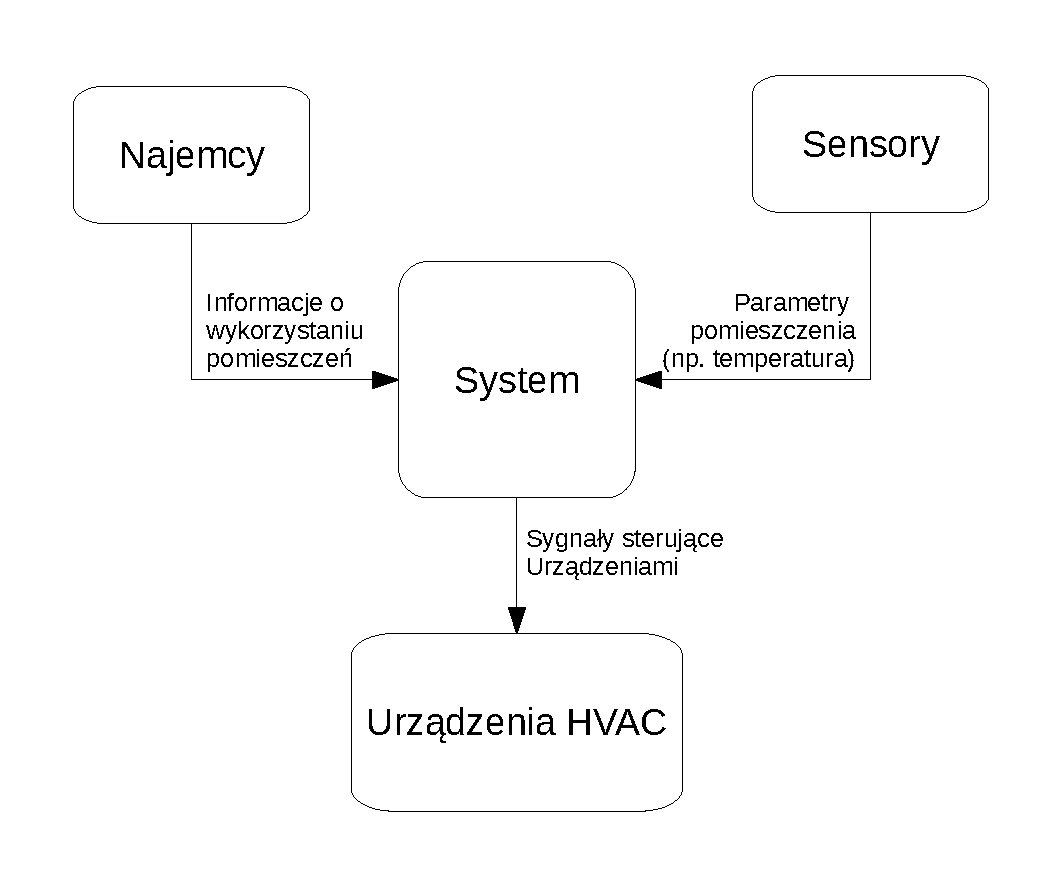
\includegraphics[width=0.7\textwidth]{./diagrams/GeneralContextDiagram.pdf}
    \caption{Kontekst systemu}
    \label{fig:generalContextDiagram}    
\end{figure}
 

Kalendarze firmowe są głównym źródłem informacji, w których pomieszczeniach i w jakich godzinach, odbywają się spotkania. Można wyobrazić sobie inne źródła, jak np. lokalizacja pracowników przypisanych do pomieszczenia. 
Jednak implementowany system będzie skupiał się głównie na wydarzeniach firmowych, jako że są mniej dynamiczne i można za ich pomocą zamodelować również np. spóźniającego się pracownika przesuwając godzinę spotkania.

System będzie sterował urządzeniami HVAC poprzez aktuatory (urządenia pozwalające komputerowi wpływać na stan świata rzeczywistego), które mogłyby składać się z mikrokomputerów z portami podczerwieni lub komunikacją radiową (Bluetooth czy WiFi.)
Aktuatory wyręczałyby użytkowników w prawidłowym ustawianiu urządzeń.
Przy ręcznym ustawianiu komfortowej temperatury przez człowieka zwykle odbywa się to na początku spotkania, gdy uczestnicy uznają, że warunki w pomieszczeniu nie odpowiadają ich wymaganiom. 
Aby jak najszybciej pozbyć się tego uczucia, włączają najmocniejszy, lecz nie koniecznie najbardziej oszczędny, tryb w klimatyzatorach.

Oszczędność z zastosowania systemu będzie przychodzić z uruchomienia klimatyzatorów przed spotkaniem w najbardziej ekonomicznym wariancie tak, aby uczestnicy mieli komfortowe warunki od początku aż do końca spotkania. 

Do wyliczenia, ile czasu wcześniej należy uruchomić urządzenia, potrzebne są matematyczne modele zjawisk, takich jak wymiana ciepła. 
Tworzeniem precyzyjnych modeli takich zajwisk zajmują się inne dziedziny techniki - ogrzewnictwo oraz chłodnictwo. 
Jako, że opracowanie dokładnych modeli jest poza zakresem tej pracy system będzie korzystał z modelu uproszczonego. 

\chapter{Analiza biznesowa}
\section{Omówienie zagadnienia}
W większości budynków biurowych zamontowane są klimatyzatory, które zapewniają komfortowe warunki pracy osób przebywających w biurach. 
Ilość prądu potrzebnego do funkcjonowania sieci takich urządzeń jest sporą częścią miesięcznych kosztów dla właściciela budynku.

Przy ręcznym ustawianiu komfortowej temperatury przez człowieka zwykle odbywa się to na początku spotkania gdy uczestnicy uznają, że warunki w pomieszczeniu nie odpowiadają ich wymaganiom. Aby jak najszybciej pozbyć się tego uczucia włączają najmocniejszy, lecz nie koniecznie najbardziej oszczędny, tryb w klimatyzatorach.

Założeniem implementowanego w tej pracy systemu jest ustalanie temperatury komfortu przed spotkaniem i uruchomienie klimatyzatorów przed spotkaniem w najbardziej ekonomicznym wariancie, tak aby uczestnicy mieli komfortowe warunki od początku spotkania i utrzymanie ich przez całe spotkanie. 

Głównym źródłem informacji w których pomieszczeniach i w jakich godzinach odbywają się spotkania są kalendarze firmowe. Można wyobrazić sobie inne źródła takie jak lokalizacja pracowników przypisanych do pomieszczenia, jednak implementowany system będzie skupiał się głównie na wydarzeniach firmowych, jako że są mniej dynamiczne i można za ich pomocą zamodelować również np. spóźniającego się pracownika przesuwając godzinę spotkania.

Przewidzieć ile czasu wcześniej należy uruchomić urządzenia i w jakim trybie można za pomocą matematycznych modeli. Przygotowanie dokładniejszych modeli nie mieści się w zakresie pracy, przyjęto zatem prosty model opierający się o moc i wydajność urządzeń. 

\section{Analiza wymagań systemu}
Przy założeniu ewentualnej późniejszej rozbudowy systemu lub przeniesienia go na inny język programowania system musiał spełniać następujące wymagania:

\subsection*{Możliwość dodania nowych parametrów pomieszczenia}
Dodanie nowych parametrów takich jak wilgotność czy nasłonecznienie pozwalałoby udoskonalić model temperatur i zbliżyć go do rzeczywistego modelu fizycznego.

Jednocześnie dodanie takich parametrów jak poziom tlenu w pomieszczeniu dawałby możliwość sprawdzenia czy osobom w pomieszczeniu nie jest zbyt duszno oraz przewietrzenia pomieszczenia za pomocą dostępnych urządzeń.

Oczywiście każde dodanie takiego parametru wiązałoby się z nowym typem sensora i w niektórych przypadkach aktuatora o ile badane zajwisko zmianiałoby się na tyle wolno, że moglibyśmy na nie oddziałowywać.

\subsubsection*{Parametryzacja i podmiana modeli}
Możliwość parametryzacji model pozwoliłaby dostrajać modele i poprawić precyzję działania i sugesti systemu.
Podmiana modeli umożliwiłaby aktualizację parametrów modelu lub podmianę na inaczej skonstruowany model (np. przewidujący temperatury z innych parametrów pomieszczenia) bez wyłączania systemu . 

\subsection*{Możliwość podpięcia różnych źródeł danych}
W różnych firmach używa się różnych systemów do ustalania terminów spotkań czy rezerwacji sal np. Microsoft Exchange Server czy IBM Domino.
System powinien pozwalać na dopisanie adaptera zajmującego się przekazywaniem wydarzeń do systemu HVAC i uniezależnianiem go od źródła danych.

\subsection*{Możliwość zbadania stanu systemu}
Dla celach diagnostycznych oraz aby dostroić modele potrzebne są dane o stanie urządzeń oraz dane z samego systemu HVAC. Musi zatem istnieć sposób, aby w łatwy sposób połączyć się z systemem HVAC i zerbać informacje o jego stanie.

\section{Analiza wymagań aplikacji symulatora}
Użycie rzeczywistych urządzeń HVAC w celu sprawdzenia poprawności działania systemu nie było możliwe w ramach tej pracy ze względu na kosztowność i czasochłonność tej metody. 

Potrzebny był zatem symulator który zawierałby w sobie system HVAC oraz interfejs użytkownika umożliwiający interakcję z systemem. Taki symulator powinien też pozwalać na przyspieszenie czasu w symulowanym systemie, ograniczyć czas potrzebny na testowanie.

Aby móc wykonywać powtarzalne próby wydajnie potrzebne były:

\subsection*{Symulacja upływu czasu}
Aby nie czekać na wynik działania systemu po np. dwóch godzinach, system powinien pozwalać na przeskalowanie czasu upływającego w systemie np. jedna sekunda czasu rzeczywistego to 5 minuty czasu symulatora.

\subsection*{Mechanizm ładowania schematu budynku}
Aplikacja symulatora powinna pozwalać na zapisanie i ponowne załadowanie właściwości pomieszczeń wraz ze stanem urządzeń zanjdujących się w nim.

\subsection*{Silnik scenariuszy}
Scenariusze czyli lista sygnałów które odbiera system o określonym czasie. Np. podniesienie się temperatury czy przesunięcie spotkania. Za pomocą odtwarzalnych scenariuszy możemy wielokrotnie testować zachowanie systemu w tych samych warunkach, ale np. z innymi parametrami w modelu temperatury.

\section{Model aktorów}
Model aktorów to model równoległości oparty oparty o aktorów którzy przesyłają między sobą wiadomości.
Model ten zakłada każdy z aktorów jest samodzielną jednostką z kolejką wiadomości. Wiadomości sa przetwarzane po jednej na raz. W ramach przetwarzania mogą nastąpić zmiana stanu wewnętrznego aktora lub wysłanie jednej lub więcej wiadomości do jednego lub więcej aktorów. 

Model zakłada jak najmniejszą odpowiedzialność pojedyńczego aktora, aby umożliwić jak najwyższą równogległość i skalowalność.

\section{Przegląd rozwiązań agentowych dla środowska .NET}
\subsection{Boris.NET}
Boris jest biblioteką do tworzenia systemów agentowych stworzoną w takcie badania metod projektowania systemów agentowych w Teesside University, Wielka Brytania. Protokół Borisa pozwala na łączenie w jeden system agentów napisanych za pomocą różnych języków takich jak C++, Lisp czy Java. 

Boris.NET jest biblioteką napisaną przez Aliego Bojarpour do obsługi biblioteki Boris za pomocą języków \csh i \fsh. 

Elastyczność Borisa pod względem ilości obsługiwanych jest cenną cechą, gdyż pozwalałaby na pisanie adapterów i dodatkowych funkcjonalności przez różne zespoły. 
Niestety ani Boris ani Boris.NET nie są projektami open-source co uniemożliwia analizę i poznanie mechanizmów wewnętrznych biblioteki. Podobnie rzecz ma się ze wsparciem społeczności, która ogranicza sie do osób ze środowiska akademickiego.

Brak też obszernej dokumentacji, która jest potrzebna przy poznawaniu nowego modelu oprogramowania jakim jest system agentowy.

W SEKCJACH PONIŻEJ POJAWIĄ SIĘ TREŚCI NA PODSTAWIE
https://github.com/akka/akka-meta/blob/master/ComparisonWithOrleans.md
\subsection{Orleans}


\subsection{Akka.net}


\subsection{Podobieństwa między Akka.net i Orelans}


\subsection{Różnice między Akką.net i Orelans}


\subsection{Uzasadnienie wyboru Akka.net}
\chapter{Systemy agentowe}
Koncepcja systemów agentowych wywodzi się z idei rozproszonej sztucznej inteligencji (DAI - Distributed Artificial Inteligence.)

W najogólniejszej definicji agenci to programy, które działają w imieniu użytkownika. Akcje mogą być proste jak zebranie lub przesłanie danych, ale mogą też zawierać elementy negocjacji z innymi agentami czy podejmowania decyzji. \cite{bib:agenciNazewnictwo}

Systemy agentowe stosuje się w miejscach gdzie ważna jest skalowalność oraz potrzeba dużego rozproszenia systemu. Przykładami mogą być systemy giełdowe gdzie każdy makler ma swojego agenta, który w imieniu właściciela będzie zgłasza chęć sprzedaży lub kupna akcji. Taki agent mógłby też negocjować ceny.

\section{Model aktorów}
Model aktorów to model równoległości oparty na koncepcji agentów posiadających wewnętrzny stan, którzy przesyłają między sobą wiadomości.
Był to pierwszy koncept, który zapoczątkował rozwój systemów agentowych.
\cite{bib:agenciNazewnictwo}

Model ten zakłada, że każdy z aktorów jest samodzielną jednostką posiadającą kolejkę wiadomości. Wiadomości sa przetwarzane po jednej na raz w kolejności, w której przyszły. W ramach przetwarzania mogą nastąpić zmiana stanu wewnętrznego aktora lub wysłanie jednej lub więcej wiadomości do jednego lub więcej aktorów. Model zakłada jak najmniejszą odpowiedzialność pojedyńczego aktora, aby umożliwić jak najwyższą równogległość i skalowalność. 

Systemy aktorów znajdują zastosowanie w grach, komunikatorach oraz wszędzie tam gdzie, duża liczba agentów często komunikuje się między sobą. \cite{bib:akkaUseCases}

\section{Przegląd rozwiązań agentowych dla środowska .NET}
Autor posiada ponad 5 lat doświadczenia w pisaniu aplikacji w środowisku .NET. 
Dlatego postanowił, że system zarządzania urządzeniami HVAC zostanie napisany w języku \csh, aby skupić się na poznawaniu zasad budowania systemów agentowych, a nie na nauce składni innych, mniej znanych mu języków programowania. 

W ciągu ostatnich lat pojawiło się kilka rozwiązań .NETowych dedykowanych do tworzenia systemów agentowych. W momencie rozpoczynania projektu autor brał pod uwagę trzy biblioteki: Boris.NET, Orleans i Akka.net.

\subsection{Boris.NET}
Boris jest biblioteką do tworzenia systemów agentowych stworzoną w takcie badania metod projektowania systemów agentowych w Teesside University, Wielka Brytania. Protokół Borisa pozwala na łączenie agentów napisanych za pomocą różnych języków takich jak C++, Lisp czy Java w jeden system. Boris.NET jest biblioteką napisaną przez Aliego Bojarpour do obsługi biblioteki Boris za pomocą języków \csh i \fsh. 

Elastyczność Borisa pod względem ilości obsługiwanych jest cenną cechą, gdyż pozwalałaby na pisanie adapterów i dodatkowych funkcjonalności przez różne zespoły. 
Niestety, ani Boris, ani Boris.NET nie są projektami open-source, co uniemożliwia analizę i poznanie mechanizmów wewnętrznych biblioteki. Podobnie rzecz ma się ze wsparciem społeczności, która ogranicza sie do osób ze środowiska akademickiego. Brak też kompleksowej dokumentacji, która jest potrzebna przy poznawaniu nowej architektury oprogramowania, jaką jest podejście agentowe.

Ze względu na powyższe wady Boris.NET nie mógł zostać wybrany do implementacji systemu zarządzania urządzeniami HVAC.

\subsection{Orleans}
Orleans to biblioteka pozwalająca na pisanie rozproszonych aplikacji stworzona przez Microsoft Research.
Powstała z myślą o osobach zaczynających pracę z systemami agentów. 
Orleans stworzyło własny model oparty na ziarnach (ang. grains) rozproszonych pomiędzy silosami. Każdy silos jest najczęściej oddzielnym serwerem.
  
\subsection{Akka.net}
Akka.net jest portem javowej biblioteki Akka, służącej do tworzenia systemów aktorów. 
Co kilka miesięcy wydawana jest nowa wersja biblioteki rozszerzona o nowe możliwości. 
Aktorzy są połączeni w drzewiastą strukturę, jednak to nie ogranicza ich możliwości wysyłania wiadomości. 

\section{Porównanie Akka.net i Orleans}
Tabela \ref{tab:AkkaVsOrleans} przedstawia porównianie bazujące na przeglądzie dr. Rolanda Kuhna \cite{bib:AkkaVsOrleans}, pozwalające ocenić, które rozwiązanie bardziej nadaje się do realizacji założeń projektu. Raport porównywał biblioteki skupiając się na tworzeniu systemów aktorów i poniższe porównanie przyjmie ten sam kontekst.

\subsection*{Kontrola nad systemem i lokalizacją aktorów}
Niektóre z możliwości Orleans mogą być interesujące dla osób zaczynających z programowaniem równoległym. 
Pisanie kodu, który ukrywa rozproszenie systemu jest dużym ułatwieniem. 
Wiele rzeczy dzieje się automatycznie lub nie mamy na nie wpływu. 
Pod tym względem Akka.net najbardziej różni się od Orleans. Wymaga się znajomości założeń, które przyjęli autorzy biblioteki. W zamian programiści mają pełną kontrolę nad tym, co dzieje się w systemie.

W projektowanym systemie ważne są między innymi lokalizacja aktorów (aby wysyłać sygnały do klimatyzatorów np. podczerwienią lub bluetooth) oraz możliwość ustrukturyzowania systemu. 
Takie możliwości daje Akka.net. Orleans jest dobry do zastosowań czysto obliczeniowych, jednak pewnych wymaganiach jego konfiguracja byłaby uciążliwa lub wręcz niemożliwa do zrealizowania.

\subsection*{Wsparcie społeczności}
Kolejnym argumentem za wykorzystaniem Akka.net jest jej cykl rozwoju.
Akka.net jest wspierana przez firmę Petabridge, której pracownicy dodają nowe funkcjonalności oraz konsultują ze społecznością rozwój Akka.net jak i oryginalnej Akki. 

Społeczność Orleans od września 2016 opracowuje nową wersję biblioteki \cite{bib:Orleans2}. Nie został podany zakres zmian w API, które zajdą wraz z tą aktualizacją. 

\subsection*{Kolejność dostarczania wiadomości}
W Akka.net kolejność dostarczenia wiadomości jest zachowywana dla każdej pary aktorów. Nie znaczy to co prawda, że wszystkie wiadomości będą przychodzić w kolejności w jakiej zostały wysłane, ale zapobiegnie to sytuacjom, gdzie wiadomość z aktualizacją stanu sprzed chwili mogłaby nadgrać najbardziej aktualny status.

Orleans nie posiada takiego mechanizmu. Jego założeniem jest, to że ziarna wykonują zlecone im obliczenia i kolejność ich wykonywania nie powinna zaburzać ich pracy.

\subsection*{Uzasadnienie wyboru Akka.net}
Większa kontrola nad systemem, stabilność API połączone z podobieństwem struktury systemu Akka.net do struktury budynku zadecydowały o wyborze Akka.net do implementacji systemu oraz symulatora.

\begin{longtabu} to \textwidth {| X[2,l] | X[3,l] | X[3,l] |}
    \caption{Porównanie Orelans i Akka.net}
    \label{tab:AkkaVsOrleans} \\
    \hline
      \multicolumn{1}{ |c| }{Cecha} 
    & \multicolumn{1}{  c| }{Orleans} 
    & \multicolumn{1}{  c| }{Akka.net} \\ 
    \hline
    \endfirsthead
    
    \multicolumn{3}{c}
    {{\bfseries \tablename\ \thetable{} -- ciąg dalszy z poprzedniej strony}} \\ 
    \hline
      \multicolumn{1}{ |c| }{Cecha} 
    & \multicolumn{1}{  c| }{Orleans} 
    & \multicolumn{1}{  c| }{Akka.net} \\ 
    \endhead

    \hline 
    \multicolumn{3}{|r|}{{Ciąg dalszy na następnej stronie}} \\ 
    \hline
    \endfoot
    
    \hline
    \endlastfoot

    Implementowany model równoległości & 
    Model Orleans może zostać przekształcony w model aktorów, gdzie każde ziarno to jeden aktor. & 
    Akka.net w całości bazuje na koncepcji modelu aktorów. \\ 
    \hline

    Transparentność położenia aktora & 
    \multicolumn{2}{ p{12cm}| }{W obu bibliotekach aktorzy nie muszą komunikować z innymi aktorami za pomocą adresów ujawniających ich fizyczną lokalizację. Zamiast tego, używają specjalnych referencji, dzięki którym nie muszą wiedzieć, gdzie znajduje się odbiorca.} \\
    \hline

    Możliwość rozproszenia systemu & 
    \multicolumn{2}{ p{12cm}| }{Zarówno Orleans jak i Akka.net zapewniają mechanizmy pozwalające na rozproszenie systemu miedzy wieloma maszynami, a także load balancing.} \\
    \hline

    Położenie aktora & 
    Determinowane przez system lub load balancer. & 
    Można narzucić adres maszyny, na której aktor będzie pracował, za pomocą odpowiedniego pliku konfiguracyjnego. \\
    \hline

    Współdzielenie pamięci & 
    \multicolumn{2}{ p{12cm}| }{Każdy z aktorów posiada własny fragment pamięci, który nie jest współdzielony z żadnym z elementów systemu aktorów.} \\
    \hline

    Przydzielanie wątków &
    \multicolumn{2}{ p{12cm}| }{Każdy aktor jest obsługiwany przez jeden wątek. Obie biblioteki nie pozwalają na wykonywanie zadań jednego aktora przez dwa równoległe wątki.} \\
    \hline 

    Zapisywanie stanu aktorów &
    \multicolumn{2}{ c| }{Oba systemy pozwalają za zapisanie stanu aktorów poza systemem.} \\
    & Stan aktorów jest zapisywany w snapshotach - zrzutach stanu ziaren.
    & Stan elementów systemu jest zapisywany za pomocą logu zdarzeń. Log pozwala też na stworzenie snapshotów. \\
    \hline 

    Serializacja wiadomości & 
    Wiadomości są zawsze serializowane. &
    Wiadomości są serializowane, gdy opuszczają lokalny system aktorów. \\
    \hline

    Tworzenie aktorów & 
    Aktorzy są tworzeni automatycznie wtedy, kiedy są potrzebni. & 
    Wymaga jawnego tworzenia aktorów. \\
    \hline

    Kontrola cyklu życia aktora & 
    Cykl życia aktora nie jest kontrolowany przez programistę. Może on jedynie podpiąć się do zdarzeń z cyklu życia. & 
    Pełna kontrola cyklu życia aktorów, włącznie z przesyłaniem wiadomości wyłączających aktorów.\\
    \hline
   
    Styl programowania & 
    Przypominający tradycyjne programowanie obiektowe z wykorzystaniem interfejsów. Na podstawie napisanego kodu generowany jest kod ziaren. & 
    Aktorzy są oddzielnymi klasami bez powiązań między sobą. Ich pisanie sprowadza się do pisania reakcji na otrzymane wiadomości.\\
    \hline

    Obsługa wyjątków & 
    Wyjątki są traktowane jako błędy w systemie. & 
    Wyjątki są traktowane jako informacja do przekazania aktorowi-rodzicowi. Od niego zależy jak zostanie potraktowany wyjątek. \\
    \hline

    Niezawodoność dostarczania wiadomości & 
    Nie zapewnia odczytu wiadomości w kolejności w jakiej przyszły.
    & Zapewnia odczyt wiadomości w kolejności w jakiej przyszły na poziomie par aktorów. \\
    & \multicolumn{2}{ c| }{Każda wiadomość jest dostarczana co najmniej raz.} \\
    \hline 
\end{longtabu}
% \end{longtable}
% \end{center}

\part{Opis proponowanego rozwiązania}
\chapter{Struktura systemu zarządzania urządzeniami}

\section{Obraz ogólny i kontekst działania systemu}

W najogólniejszym obrazie, system odpowiada za przetwarzanie danych zebranych z sensorów rozmieszczonych w pomieszczeniach oraz informacji zapisanych w kalendarzach firm (syngały te mogą dotyczyć takich rzeczy jak np. zmiana godziny rozpoczęcia spotkania) na sygnały sterujące wysyłane do urządzeń HVAC aby zachować w pomieszczeniach odpowiednie parametry, takie jak temperatura czy poziom ilości tlenu w powietrzu. \seefigure{generalContextDiagram}

\section{Moduły systemu}
DIAGRAM MODUŁÓW SYSTEMU
% \input{./diagrams/systemModules}

W budowie samego systemu zarządzania urządzeniami HVAC możemy wyróżnić kilka modułów.
\begin{enumerate}
    \item Modele - zestaw abstrakcji modelujących realy świat, użyty do budowy pozostałych modułów.  
    \item Jednostki - zestaw klas do budowy aktorów odpowiedzialnych za komunikację z sensorami i aktuatorami.
    \item Odczyt i kontrola parametrów - moduł zawierający matematyczny model zmiany temperatury wraz z aktrorami odpowiedzialnynmi za wysyłanie klimatyzatorom odpowiednich dyspozycji.
    \item Symulacja zmiany parametrów - matematyczne modele pozwalające przewidzieć zmiany parametrów wywołane działaniem aktuatorów.
    \item Źródła wymagań - zestaw adapterów przetwarzających dane nadesłane do systemu na wymagania dla poszczególnych parametrów. 
    \item Zarządzanie Pomieszczeniem - moduł odpowiedzialny za zarządzanie komunikacją pomiędzy sensorami a aktuatorami. 
\end{enumerate}

Należy też wyróżnić moduł aplikacji hostującej system aktorów. 
Może być to zarówno aplikacja desktopowa jak i webowa. 

\section{Architektura systemu aktorów}
Systemy aktorów w akka.net mają strukturę drzewiastą. 
Każdy aktor jest dzieckiem aktora głównego lub innego aktora. 

\begin{figure}[ht!]
    \centering
    \tikzset{
        edge from parent fork down,        
        level distance = 2cm,
        minimum height=8mm,
        every tree node/.style={draw, rectangle, rounded corners, align=center}}
    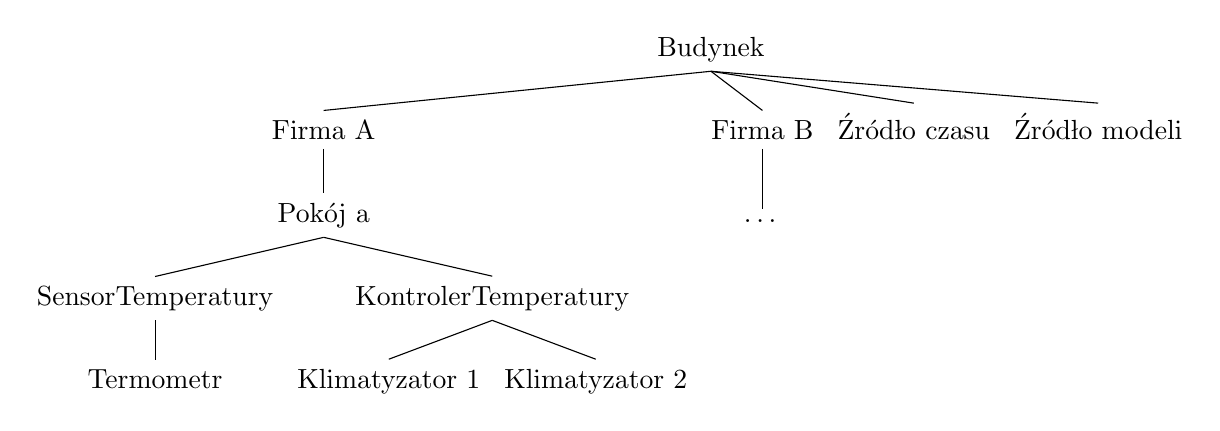
\begin{tikzpicture}[]
    \Tree 
        [.Budynek   
            [.{Firma A} 
                [.{Pokój a}   
                    [. {Sensor\\Temperatury} 
                        Termometr 
                    ]
                    [.{Kontroler\\Temperatury} 
                        {Klimatyzator 1} 
                        {Klimatyzator 2}
                    ]                    
                ]
            ]
            [.{Firma B} 
                {\ldots}
            ]
            {Źródło czasu}
            {Źródło modeli}
        ]        
    \end{tikzpicture}
    \caption{Schemat systemu aktorów}
\end{figure}
 

Aktor główny symbolizuje modelowany budynek.
Jego dziećmi są aktorzy firm, którzy odpowiadają za odświeżanie informacji z kalendarzy i przechowywanie ewentualnych domyślnych wartości parametrów pomieszczeń.

Każda firma ma pod sobą kilku aktorów odpowiedzialnych za przypisane im pomieszczenia.
Aby móc wpływać na parametry pomieszczenia, jego aktor ma dostęp do danych o pomieszczeniu od agentów sensorów oraz może wysłać sygnały kontrolne do urządzeń za pomocą aktorów kontrolerów.

Oba powyższe rodzaje aktorów łączą się z urządzeniami, odpowiednio sensorami i aktuatorami.

Dodatkowo oprócz opisanej struktury, w systemie powienien występować co najmniej jeden aktor będący źródłem czasu oraz jeden będący źródłem modeli parametrów pomieszczenia.

\chapter{Wzorce projektowe wykorzystane podczas realizacji projektu}
\section{Rekwizyty}
Rekwizyt (ang. props) to obiekt w akka.net pozwalający na przechowywanie sposobu tworzenia obiektu aktora. 
Są wykorzystywane przy zarówno tworzeniu jak i ponownym uruchamianiu aktorów po nastąpieniu nieobsłużonego wyjątku.
Tylko one mają bezpośredni dostęp do kontruktora aktora. W momencie tworzenia aktora wykorzystywany jest obiekt rekwizytów i wywoływane jest ukryte wewnątrz wyrażenie z konstruktorem.

\section{Model subskrypcyjny}
Model subskrypcyjny (ang. subscribe/unsubscribe) to sposób komunikacji między agentami. Składa się z właściciela subskrypcji oraz subskrybentów. 
\definition{Subskrypcja to wiadomość rozsyłana przez jej właściciela do wszystkich którzy się złosili.}
\definition{Subskrybentem nazywamy agenta, który zgłosił właścicielowi subskrypcji chęć otrzymywania subskrypcji.

\begin{figure}[ht!]
    \centering
    \begin{sequencediagram}
        \newinst[2]{Owner}{Właściciel subskrybcji}{}
        \newinst[2]{Nowy}{Nowy subskrybent}{}
        \newinst[2]{Stary}{Subskrybent}{}

        \begin{mess}{Nowy}{Subscibe}{Owner}\end{mess}
        \begin{mess}{Owner}{Newsletter}{Nowy}\end{mess}
    \end{sequencediagram}
    \caption{Schemat dodawania subskrybenta}
    \label{fig:subscribe}
\end{figure}
 
W realizowanym systemie właściciel subskrypcji wysyła ostatnią rozesłąną subskrypcję do agenta, który zapisał się na subskrypcję. Dzięki temu dopiero co zapisany agent nie musi czekać na kolejny syngał inicjalizujący rozesłanie subskrypcji.
 
\begin{figure}[ht!]
    \centering
    \begin{sequencediagram}
        \newinst[1]{TriggerSource}{Źródło sygnału}{}
        \newinst[2]{Owner}{Właściciel subskrybcji}{}
        \newinst[1]{Sub1}{Subskrybent A}{}
        \newinst[1]{Sub2}{Subskrybent B}{}

        \begin{mess}{TriggerSource}{Trigger}{Owner}\end{mess}
        \begin{mess}{Owner}{Newsletter}{Sub1}\end{mess}
        \begin{mess}{Owner}{Newsletter}{Sub2}\end{mess}
    \end{sequencediagram}
    \caption{Schemat rozsyłania subskrypcji}
    \label{fig:subscriptionTrigger}
\end{figure}
 
Właściciel subskrypcji może rozsyłać subskrypcję zarówno na sygnał czasowy jak i sygnał przychodzący z zewnątrz. 

\section{Udostępnianie informacji o stanie aktora}
Aby móc w łatwy sposób odczytywać stan wewnętrzny systemu, większość jego aktorów dziedziczy po specjalnie napisanym typie aktora ???DebugableActor???. Ta klasa pozwala na przygotowanie informacji, która będzie rozsyłana za pomocą specjalnej subskrypcji diagnostycznej. Zadanie wybrania momentów w których rozsyłana jest subskrypcja należy do osoby rozszerzającej tą klasę. 

Metody dostępne do rozszerzenia lub użycia w klasie ???DebuggableActor???
\begin{enumerate}
    \item GenerateInternalState() - tworzy obiekt przedstawiający stan wewnętrzny aktora (metoda do rozszerzenia). 
    \item InformAboutInternalState() - rozsyła subskrypcję stanu wewnętrznego do wszystkich diagnostycznych subskrybentów.
    \item InformDebugSubscribers(object x) - Pozwala rozesłać do subskrybentów diagnostyczych inną wiadomość niż tą generowaną za pomocą GenerateInternalState()
    \item SetInternalStatus() - Metoda pozwalająca na nadgranie statusu wewnętrznego aktora np. w celu testowania. Domyślnie nie zmienia stanu aktora a jedynie wywołuje metodę InformAboutInternalState(). (metoda do rozszerzenia)
\end{enumerate}

\section{Aktor-pomost}
Aktor-pomost (ang. BridgeActor) to aktor pośredniczący w komunikacji pomiędzy interfejsem użytkownika symulatora a właściwym agentem z właściwego systemu. 

\subsection*{Tworzenie agenta-pomostu}
Powinien mieć przypisanego tylko jednego agenta z systemu i tylko jeden model widoku z interfejsu użytkownika. Przy tworzeniu pomost zapisuje się na subskrypcję diagnostyczną, ab odbierać informacje o wszelkich możliwych zmianach stanu aktora, do którego jest pośrednikiem.
\begin{figure}[ht!]
    \centering
    \begin{sequencediagram}
        \newinst[]{ViewModel}{Model widoku}{}
        \newinst[3]{Bridge}{Aktor-pomost}{}
        \newinst[3]{Actor}{Aktor}{}

    \begin{mess}{ViewModel}{<Model widoku,Adres Aktora>}{Bridge}\end{mess}
    \begin{mess}{Bridge}{DebugSubscribe}{Actor}\end{mess}
    \begin{mess}{Actor}{InternalStatus}{Bridge}\end{mess}
    \end{sequencediagram}
    \caption{Schemat tworzenia aktora-pomostu}
\end{figure}
 

Głównym zadaniem aktora-pomostu jest przesyłanie wiadomości do aktorów wewnątrz systemu zarządzającego urządzeniami oraz aktualizacja danych widocznych w aplikacji.

\subsection*{Przekazywanie wiadomości}
\begin{figure}[ht!]
    \centering
    \begin{sequencediagram}
        \newinst[1]{UI}{Interfejs użytkownika}{}
        \newinst[1]{ViewModel}{Model widoku}{}
        \newinst[1]{Bridge}{Aktor-pomost}{}
        \newinst[1]{Actor}{Aktor}{}

    \begin{mess}{UI}{AddSensor Button Click}{ViewModel}\end{mess}
    \begin{mess}{ViewModel}{AddSensor}{Bridge}\end{mess}
    \begin{mess}{Bridge}{AddSensor}{Actor}\end{mess}
    \end{sequencediagram}
    \caption{Schemat przekazywania wiadomości przez aktora-pomost}
    \label{fig:bridgeActorForwarding}
\end{figure}
 
Po akcji użytkownika, model widoku przesyła wiadomość do aktora-pomostu, który przekazuje wiadomość dalej do przypisanego mu agenta. Czasami model widoku może oczekiwać odpowiedzi od systemu (tzw. Ask) jednak jest to widoczne tylko na poziomie widoku modelu i blokuje tylko wątek odpowiedzialny za obsługę danego kliknięcia/edycji.

\subsection*{Aktualizacja interfejsu użytkownika}
\begin{figure}[ht!]
    \centering
    \begin{sequencediagram}
        \newinst[1]{UI}{Interfejs użytkownika}{}
        \newinst[1]{ViewModel}{Model widoku}{}
        \newinst[1]{Bridge}{Aktor-pomost}{}
        \newinst[1]{Actor}{Aktor}{}

    \begin{mess}{Actor}{Room Status}{Bridge}\end{mess}
    \begin{mess}{Bridge}{UpdateFromStatus}{ViewModel}\end{mess}
    \begin{mess}{ViewModel}{PropertyChanged}{UI}\end{mess}
    \end{sequencediagram}
    \caption{Schemat aktualizowania interfejsu użytkownika przez aktora-pomost}
\end{figure}
 
Wiadomość od agenta z systemu przychodzi do agenta-pomostu. Ten, wywołuje przygotowaną w modelu widoku metodę do aktualizacji wartości wyświetlanych.
Po wykonaniu metody uruchamia się zdarzenie aktualizujące wyświetlane wartości w interfejsie użytkownika.

\section{Wiadomości typu Request/Update/Value}
Do wygodnej obsługi odpytywania systemu oraz możliwości podmiany parametrów w symulatorze powstał schemat nazewnictwa wiadomości.
\begin{itemize}
    \item Value - Wiadomość zawierająca wartość parametru.
    \item Request - Wezwanie do wysłania wartości danego parametru. Odbiorca powinien odesłać wiadomość typu Value.
    \item Update - Wiadmość zlecająca nadpisanie wartości danego parametru u odbiorcy na wartość podaną w wiadomości.
\end{itemize}


\section{Obiekty typu Wymaganie/Praca/Zadanie}
Obsługa oczekiwanych parametrów została podzielona na trzy etapy. Wymagania zostają rozbite na Zadania dla kontroleró poszczególnych parametrów, a następnie modele pozwalają wyliczyć najbardziej optymalną konfigurację urządzeń, zapisaną w obiekcie Pracy. 

\begin{itemize}
    \item Wymaganie - obiekt opisujący kiedy, który parametr i jaka jego wartość jest oczekiwana.
    
    \item Zadanie - obiekt opisujący ograniczenia w których musi być spełnione Wymaganie. 

    Np. TemperatureTask to ilość czasu, obecna temperatura w pomieszczeniu i temperature jaką chcemy osiągnąć w przeciągu ww. czasu.
    
    \item Praca - obiekt określający najlepszą znalezioną konfigurację dla zadanego Zadania. 

    Np. TemperatureJob składa się z informacji: w którym trybie, od kiedy do kiedy, i na jaką temperaturę nastawić klimatyzatory.
\end{itemize}

\chapter{Aktorzy}
\section{Źródło czasu}
\section{Źródło modeli}
\section{Firma}
\section{Pomieszczenie}
\section{Symulator pomieszczenia}

\section{Komponenty}
\subsection{Komponent cykliczny}
\subsection{Komponent symulujący}
\section{Sensor}
\section{Symulator sensora}
\subsection{Symulator parametru pomieszczenia}
\section{Kontroler}
\chapter{Interakcje między aktorami}
Dla zwiększenia czytelności wszystkie diagramy w tym rozdziale traktują  interfejs użytkownika i model widoku jako całość. Są to komponenty spoza systemu aktorów łączące się z nim zawsze za pomocą aktorów-pomostów.

Dla opisu interakcji w systemie aktorów nie jest tak istotne jaki był czynnik inicjujący interakcje np klik, w porównaniu do wiadomości która przyszła do systemu.

\section{Dodawanie/usuwanie pomieszczeń}

\subsection*{Dodanie pomieszczenia}
opis
\begin{figure}[ht!]
    \centering
    \begin{sequencediagram}
        \newinst[]{A}{Client}{}
        \newinst[]{B}{ServerA}{}
        \begin{call}{A}{Call()}{B}{}
        \end{call}
    \end{sequencediagram}
    \caption{Schamat dodawania pomieszczenia}
    \label{fig:addRoom}
\end{figure}
 
\subsection*{Usunięcie pomieszczenia}
opis
\begin{figure}[ht!]
    \centering
    \begin{sequencediagram}
        \newinst[0]{UI}{\shortstack{Interfejs\\użytkownika}}{}
        \newinst[2]{Company}{Firma}{}
        \newinst[2]{Room}{Pokój}{}
        \newinst[1]{Child1}{Sensor}{}
        \newinst[1]{Child2}{Kontroler}{}
        \newinst[1]{Time}{\shortstack{Źródło\\czasu}}{}

        \begin{mess}{UI}{RemoveRoom}{Company} \end{mess}
        \begin{mess}{Company}{RemoveRoom}{Room} \end{mess}
            
        \begin{mess}{Room}{Unsubscribe}{Time} \end{mess}
        \begin{call}{Company}{}{Company}{\shortstack{Usuń pokój\\z listy}}\end{call}
            
        \begin{sdblock}{Wygaszanie aktora}{}
            \begin{mess}{Room}{Stop}{Child2} \end{mess}
            \begin{mess}{Room}{Stop}{Child1} \end{mess}
            \begin{call}{Room}{}{Room}{Stop} \end{call}
        \end{sdblock}
    \end{sequencediagram}
    \caption{Schemat usuwania pomieszczenia}
    \label{fig:removeRoom}
\end{figure}
 

\section{Dodawanie/usuwanie sensorów i kontrolerów}
\subsection*{Dodanie sensora}
opis
\begin{figure}[ht!]
    \centering
    \begin{sequencediagram}
        \newinst[]{Room}{Room}{}
        \newinst[2]{Sensor}{TemperatureSensor}{}
        \newinst[2]{Model}{ModelParams}{}
        \newinst[]{Time}{TimeSimulator}{}

        \begin{mess}{Room}{Adresy subskrypcji}{Sensor}\end{mess}

        \begin{sdblock}{Subskrypcje sensora}{}
            \begin{mess}{Sensor}{Subscibe}{Room}\end{mess}
            \begin{mess}{Sensor}{Subscibe}{Model}\end{mess}
            \begin{mess}{Sensor}{Subscibe}{Time}\end{mess}
        \end{sdblock}

        \begin{sdblock}{Odpowiedzi na subskrupcje}{}
            \begin{mess}{Time}{TimeChanged}{Sensor}\end{mess}   
            \begin{mess}{Model}{TemperatureModel}{Sensor}\end{mess}
            \begin{mess}{Room}{RoomStatus}{Sensor}\end{mess}
        \end{sdblock}
                
        \begin{sdblock}{Podpięcie sensora}{}
            \begin{mess}{Sensor}{SensorAvaliable}{Room}\end{mess}
            \begin{mess}{Room}{Subscribe}{Sensor}\end{mess}
            \begin{mess}{Sensor}{TemperatureValue}{Room}\end{mess}
        \end{sdblock}
    \end{sequencediagram}
    \caption{Schemat dodawania symulatora sensora do pomieszczenia}
    \label{fig:addTemperatureSensor}
\end{figure}
 
\subsection*{Usunięcie sensora}
opis
\begin{figure}[ht!]
    \centering
    \begin{sequencediagram}
        \newinst[]{UI}{\shortstack{Interfejs\\użytkownika}}{}
        \newinst[]{Room}{Room}{}
        \newinst[2]{Sensor}{TemperatureSensor}{}
        \newinst[2]{Model}{ModelParams}{}
        \newinst[]{Time}{TimeSimulator}{}


        \begin{mess}{UI}{RemoveSensor}{Room}\end{mess}
        \begin{mess}{Room}{RemoveSensor}{Sensor}\end{mess}

        \begin{call}{Room}{}{Room}{Usuń sensor z listy}\end{call}            

        \begin{sdblock}{Subskrypcje sensora}{}
            \begin{mess}{Sensor}{Unsubscibe}{Room}\end{mess}
            \begin{mess}{Sensor}{Unsubscibe}{Model}\end{mess}
            \begin{mess}{Sensor}{Unsubscibe}{Time}\end{mess}
        \end{sdblock}

    \begin{call}{Sensor}{}{Sensor}{Stop}\end{call}
    \end{sequencediagram}
    \caption{Schemat usuwania symulatora sensora z pomieszczenia}
    \label{fig:removeTemperatureSensor}
\end{figure}
 
\subsection*{Dodanie kontrolera}
opis
\begin{figure}[ht!]
    \centering
    \begin{sequencediagram}
        \newinst[0]{Room}{Pokój}{}
        \newinst[2]{Controller}{\shortstack{Kontroler\\temperatury}}{}
        \newinst[2]{Model}{\shortstack{Źródło\\modeli}}{}
        \newinst[]{Time}{\shortstack{Źródło\\czasu}}{}

        \begin{mess}{Room}{Adresy subskrypcji}{Controller}\end{mess}

        \begin{sdblock}{Subskrypcje kontrolera}{}
            \begin{mess}{Controller}{Subscibe}{Room}\end{mess}
            \begin{mess}{Controller}{Subscibe}{Model}\end{mess}
            \begin{mess}{Controller}{Subscibe}{Time}\end{mess}
        \end{sdblock}

        \begin{sdblock}{Odpowiedzi na subskrupcje}{}
            \begin{mess}{Time}{TimeChanged}{Controller}\end{mess}   
            \begin{mess}{Model}{TemperatureModel}{Controller}\end{mess}
            \begin{mess}{Room}{RoomStatus}{Controller}\end{mess}
        \end{sdblock}
                
        \begin{sdblock}{Podpięcie kontrolera}{}
            \begin{mess}{Controller}{SensorAvaliable}{Room}\end{mess}
            \begin{mess}{Room}{Subscribe}{Controller}\end{mess}
            \begin{mess}{Controller}{TemperatureValue}{Room}\end{mess}
        \end{sdblock}
    \end{sequencediagram}
    \caption{Schemat dodawania kontrolera temperatury do pomieszczenia}
    \label{fig:addTemperatureController}
\end{figure}
 
\subsection*{Usunięcie kontrolera}
opis
\begin{figure}[ht!]
    \centering
    \begin{sequencediagram}
        \newinst[]{UI}{\shortstack{Interfejs\\użytkownika}}{}
        \newinst[]{Room}{Room}{}
        \newinst[2]{Controller}{TemperatureController}{}
        \newinst[2]{Model}{ModelParams}{}
        \newinst[]{Time}{TimeSimulator}{}


        \begin{mess}{UI}{RemoveSensor}{Room}\end{mess}
        \begin{mess}{Room}{RemoveSensor}{Controller}\end{mess}

        \begin{call}{Room}{}{Room}{Usuń kontroler z listy}\end{call}            

        \begin{sdblock}{Subskrypcje kontrolera}{}
            \begin{mess}{Controller}{Unsubscibe}{Room}\end{mess}
            \begin{mess}{Controller}{Unsubscibe}{Model}\end{mess}
            \begin{mess}{Controller}{Unsubscibe}{Time}\end{mess}
        \end{sdblock}

    \begin{call}{Controller}{}{Controller}{Stop}\end{call}
    \end{sequencediagram}
    \caption{Schemat usuwania kontrolera temperatury z pomieszczenia}
    \label{fig:removeTemperatureController}
\end{figure}
 

\section{Dodawanie/usuwanie urządzeń}
\subsection*{Dodanie urządzenia}
\begin{figure}[!htbp]
    \centering
    \begin{sequencediagram}
        \newinst[]{UI}{\shortstack{Interfejs\\użytkownika}}{}
        \newinst[]{Room}{Pokój}{}
        \newinst[]{Controller}{\shortstack{Kontroler\\temperatury}}{}
        \newinst[]{JobScheduler}{Planista}{}

        \begin{mess}{UI}{DeviceDefinition}{Room}\end{mess}
        \begin{mess}{Room}{DeviceDefinition}{Controller}\end{mess}

        \begin{call}{Controller}{}{Controller}{\shortstack{Dodaj urządzenia do listy}}\end{call}

        \begin{mess}{Controller}{TemperatureTask}{JobScheduler}\end{mess}
            
        \begin{mess}{JobScheduler}{Execution Plan}{Controller}\end{mess}              
        \begin{sdblock}{Jeżeli plan zakłada natychmiastową reakcję}{}
            \begin{call}{Controller}{}{Controller}{\shortstack{Przelacz urządzenia na\\odpowiedni tryb}}\end{call}
            \begin{mess}{Controller}{DevicesStatus}{Room}\end{mess}
        \end{sdblock} 
    \end{sequencediagram}
    \caption{Schemat dodawania urządzenia HVAC do pomieszczenia}
    \label{fig:addDevice}
\end{figure}
 
\subsection*{Usunięcie urządzenia}
\begin{figure}[ht!]
    \centering
    \begin{sequencediagram}
        \newinst[]{UI}{\shortstack{Interfejs\\użytkownika}}{}
        \newinst[]{Room}{Pokój}{}
        \newinst[2]{Controller}{\shortstack{Kontroler\\temperatury}}
        \newinst[2]{JobScheduler}{Planista}{}

        \begin{mess}{UI}{RemoveDevice}{Room}\end{mess}
        \begin{mess}{Room}{RemoveDevice}{Controller}\end{mess}
        
        \begin{mess}{Controller}{TemperatureTask}{JobScheduler}\end{mess}      
        \begin{mess}{JobScheduler}{Execution Plan}{Controller}\end{mess} 
        
        \begin{sdblock}{Jeżeli plan zakłada natychmiastową reakcję}{}
            \begin{call}{Controller}{}{Controller}{\shortstack{Przelacz urządzenia na\\odpowiedni tryb}}\end{call}
            \begin{mess}{Controller}{DevicesStatus}{Room}\end{mess}
        \end{sdblock}
    \end{sequencediagram}
    \caption{Schemat usuwania urządzenia HVAC z pomieszczenia}
    \label{fig:removeDevice}
\end{figure}
 

\section{Upływ czasu}
\subsection{Sensor/symulator sensora}
\begin{figure}[ht!]
    \centering
    \begin{sequencediagram}
        \newinst[0]{Time}{\shortstack{Źródło\\czasu}}{}
        \newinst[]{Sensor}{Sensor}{}
        \newinst[6]{Subs}{Subskrybenci}{}

        \begin{mess}{Time}{TimeChanged}{Sensor}\end{mess}
        \begin{call}{Sensor}{\shortstack{Sprawdz ile czasu upłynelo}}{Sensor}{jesli $\Delta_t$ > okres aktualizacji}\end{call}
        \begin{mess}{Sensor}{ParameterValue}{Subs}\end{mess}
    \end{sequencediagram}
    \caption{Reakcja sensora na upływ czasu}
    \label{fig:timeChangedSensor}    
\end{figure}
 
\subsection{Kontroler}
\begin{figure}[ht!]
    \centering
    \begin{sequencediagram}
        \newinst[0]{Time}{\shortstack{Źródło\\czasu}}{}
        \newinst[]{Controller}{Kontroler}{}
        \newinst[6]{Subs}{Subskrybenci}{}

        \begin{mess}{Time}{TimeChanged}{Controller}\end{mess}
        \begin{call}{Controller}{\shortstack{Sprawdz czy nie nalezy rozpoczac pracy}}{Controller}{jezeli tak, to uruchom urzadzenia}\end{call}
        \begin{mess}{Controller}{ControllerStatus}{Subs}\end{mess}
    \end{sequencediagram}
    \caption{Reakcja kontrolera na upływ czasu}
    \label{fig:timeChangedController}    
\end{figure}
 
\subsection{Scenarzysta}
\begin{figure}[ht!]
    \centering
    \begin{sequencediagram}
        \newinst[0]{Time}{\shortstack{Źródło\\czasu}}{}
        \newinst[]{Screenwriter}{Scenarzysta}{}
        \newinst[6]{Target}{\shortstack{Adresaci\\wiadomości}}{}

        \begin{mess}{Time}{TimeChanged}{Screenwriter}\end{mess}
        \begin{call}{Screenwriter}{\shortstack{Znajdz wiadomości, ktore\\nalezy wyslac w obecnej chwili}}{Screenwriter}{}\end{call}
        \begin{mess}{Screenwriter}{Wiadomość}{Target}\end{mess}
    \end{sequencediagram}
    \caption{Reakcja scenarzysty na upływ czasu}
    \label{fig:timeChangedScreenwriter}    
\end{figure}
 

\section{Zmiana wartości parametów modelu}

\section{Zmiana wartości parametów symulowanego pomieszczenia}

\section{Zmiany stanu wydarzeń w kalendarzu}
\begin{figure}[ht!]
    \centering
    \begin{sequencediagram}
        \newinst[]{Calendar}{\shortstack{Adapter do\\kalendarza}}{}
        \newinst[]{Company}{Firma}{}
        \newinst[]{Room}{Pokój}{}
        \newinst[]{Controller}{Kontroler}{}
        \newinst[]{JobScheduler}{Planista}{}

        \begin{mess}{Calendar}{CalendarEvents}{Company}\end{mess}
        
        \begin{mess}{Company}{Expectations}{Room}\end{mess}
        \begin{mess}{Room}{Expectations}{Controller}\end{mess}
        
        \begin{mess}{Controller}{Tasks}{JobScheduler}\end{mess}
        \begin{mess}{JobScheduler}{ExecutionPlan}{Controller}\end{mess}

        \begin{sdblock}{Jeżeli zmiany wymagają natychmiastowej reakcji}{}
            \begin{call}{Controller}{}{Controller} {\shortstack{Przestaw\\urządzenia}}\end{call}
            \begin{mess}{Controller}{DevicesStatus}{Room}\end{mess}
            \begin{mess}{Room}{RoomStatus}{Company}\end{mess}
        \end{sdblock}
    \end{sequencediagram}
    \caption{Schemat dodawania subskrybenta}
    \label{fig:scheduling}    
\end{figure}
 
Gdy kontroler otrzyma listę wymagań przesyła ją w postaci zadania do podległego mu aktora-planisty, którego jedynym zadanim jest wykonanie obliczeń. Dzięki przekazaniu zadania podległemu aktorowi jednostka nie jest zablokowana podczas obliczeń i może wykonywać inne zadania. \seefigure{scheduling}

Czynnością wykonywaną w tym czasie mogłoby być np. okresowa weryfikacja czy zmiana wartości parametru postępuje w założonym tempie.

Po otrzymaniu od aktora-planisty definicji pracy jaką ma wykonać, kontroler ustawia odpowiednio urządzenia-aktuatory w sposób zależny od typu parametru.




\chapter{Testy}
\section{Testy w Akka.net}
Podstawowymi testami jakie można wykonać są testy jednostkowe posczególnych aktorów.
W Akka.net testy te pisze się za pomocą specjalnej paczki Akka.TestKit wystawiającej zestaw narzędzi do testowania aktorów.

Testy najczęściej mają podobną strukturę:
\begin{enumerate}
    \item Stworzenie aktora.
    \item Przesłanie mu wiadomości inicjalizujących (jeżeli jest taka potrzeba.)
    \item Wysłanie wiadomości uruchamiającej testowane zachowane aktora.
    \item Odczytanie zwróconej w.iadomości i sprawdzenie czy wartości wewnątrz zgadzają się z oczekiwaniami
\end{enumerate}
Istotne jest zauważenie różnicy w stosunku do tradycyjnych testów jednostkowych. Nie sprawdza się stanu wewnętrznego aktora, lecz jego reakcje na wiadomości.

\section{Pułapki związane z testowaniem aktorów}
\subsection{Sprawdzanie stanu wewnętrznego aktora}
Mimo tego, że Akka.TestKit udostępnia metody pozwalające na sprawdzenie stanu wewnętrznego aktora, nie jest to zalecane podejście. 
Prowadzi do sytuacji, gdzie testy zależą od wewnętrznej implementacji. 
Tak jak w tradycyjnych testach jednostkowych testuje się implementacje interfejsów, tak w Akka.net testuje się zachowania na poszczególne obsługiwane wiadomości.

\subsection{Używanie metody \lstinline{Ask} }
\lstinline{Ask<T>} jest metodą pozwalającą oczekiwać na wiadomość zwrotną z systemu aktorów danego typu \lstinline{T}.
Jest ona częścią wewnętrznych mechanizmów Akka.net i sami twórcy nie zalecają jej używania wewnątrz pisanych aktorów \cite{bib:AkkaNoAsk}. 
\lstinline{Ask<T>} nie pozwala na zmianę wątku, co w przypadku testów doprowadza do sytuacji, gdzie test zwraca błąd związany z przekroczeniem czasu oczekiwania na wiadomość zwrotną. Zamiast tego, w testach powinna występować metoda \lstinline{ExpectMsg<T>}, która zwraca pierwszą wiadomość typu \lstinline{T}, która przyjdzie do aktora testowego dostępnego w klasie \lstinline{TestKit}.  

\section{Scenariusze testowe}
Poza testami jednostkowymi, powstały też testy integracyjne łączące w jednym teście większość stworzonych aktorów. Testy te odzwierciedlają realne sytuacje spotykane w firmach wynajmujących biura. 

\subsection{Nagłe dodanie spotkania}
\begin{lstlisting}
    7:30 - w sali do spotkań panuje temperatura 25st.C
    Zaplanowane jest spotkanie na 10:30 kończące się o 12:00 z wymaganą temperaturą 21st.C
    
    8:30 - dyrektor dodaje spotkanie spotkanie z zespołem na 09:00 kończące się o 10:00 z wymaganą temperaturą 18st.C

    9:00 - w sali powinna panować temperatura 18st.C +- 0.5st.C
    
    10:00 - w sali powinna panować temperatura 18st.C +- 0.5st.C
    
    10:30 - w sali powinna panować temperatura 21st.C +- 0.5st.C
    
    12:00 - wszystkie urządzenia w sali powinny być wyłączone, 
    jako że nie ma przewidzianych innych spotkań na ten dzień
\end{lstlisting}

\subsection{Anulowanie spotkania}
\begin{lstlisting}
    7:30 - w sali do spotkań panuje temperatura 25st.C
    Zaplanowane są dwa spotkania:
     -spotkanie z klientem na 9:00 kończące się o 10:00 z wymaganą temperaturą 18st.C    
     -spotkanie zespołu na 10:30 kończące się o 12:00 z wymaganą temperaturą 21st.C
    
    8:30 - do recepcji dzwoni klient i odwołuje spotkanie
    
    9:00 - wszystkie urządzenia w sali powinny być wyłączone

    10:30 - w sali powinna panować temperatura 21st.C +- 0.5st.C

    12:00 - wszystkie urządzenia w sali powinny być wyłączone, 
    jako że nie ma przewidzianych innych spotkań na ten dzień
\end{lstlisting}

\subsection{Przesunięcie spotkania}
\begin{lstlisting}
    7:30 - w sali do spotkań panuje temperatura 25st.C
    Zaplanowane jest spotkanie na 9:00 kończące się o 12:00 z wymaganą temperaturą 18st.C
        
    8:30 - Spotkanie zostaje przesunięte na 11:00 do 14:00

    9:00 - wszystkie urządzenia w sali powinny być wyłączone
    
    11:00 - w sali powinna panować temperatura 18st.C +- 0.5st.C
   
    14:00 - wszystkie urządzenia w sali powinny być wyłączone, 
    jako że nie ma przewidzianych innych spotkań na ten dzień
\end{lstlisting}

\subsection{Przedłużenie spotkania}
\begin{lstlisting}
    7:30 - w sali do spotkań panuje temperatura 25st.C
    Zaplanowane jest spotkanie na 9:00 kończące się o 11:00 z wymaganą temperaturą 18st.C
            
    9:00 - w sali powinna panować temperatura 18st.C +- 0.5st.C
    
    10:45 - Spotkanie zostaje przedłużone do 12:00
    
    11:30 - w sali powinna panować temperatura 18st.C +- 0.5st.C
   
    12:00 - wszystkie urządzenia w sali powinny być wyłączone, 
    jako że nie ma przewidzianych innych spotkań na ten dzień
\end{lstlisting}

\subsection{Otwarcie okna - zmiana temperatury niezgodna z modelem}
\begin{lstlisting}
    7:30 - w sali do spotkań panuje temperatura 20st.C
    Zaplanowane jest spotkanie na 9:00 kończące się o 11:00 z wymaganą temperaturą 23st.C

    8:30 - Otwarcie okna powoduje spadek temperatury do 18st.C 
    
    9:00 - w sali powinna panować temperatura 23st.C +- 0.5st.C

    11:00 - wszystkie urządzenia w sali powinny być wyłączone, 
    jako że nie ma przewidzianych innych spotkań na ten dzień
\end{lstlisting}

\chapter{Symulator budynku biurowego}
Aby móc wykonywać powtarzalne próby wydajnie potrzebne były:

\section{Analiza wymagań aplikacji symulatora}
Użycie rzeczywistych urządzeń HVAC, w celu sprawdzenia poprawności działania systemu, nie było możliwe w ramach tej pracy ze względu na kosztowność i czasochłonność takiego rozwiązania. 
Potrzebny był zatem symulator który zawierałby w sobie system HVAC oraz interfejs użytkownika umożliwiający interakcję z systemem. 

\subsection*{Symulacja upływu czasu}
Symulator powinien też pozwalać na przyspieszenie czasu w symulowanym systemie, ograniczyć czas potrzebny na testowanie.
i nie czekać na wynik działania systemu po np. dwóch godzinach. System powinien pozwalać na przeskalowanie czasu upływającego w systemie np. jedna sekunda czasu rzeczywistego to 5 minut czasu symulatora.

\subsection*{Mechanizm ładowania schematu budynku}
Aplikacja symulatora powinna pozwalać na zapisanie i ponowne załadowanie właściwości pomieszczeń wraz ze stanem urządzeń zanjdujących się w nim.

\subsection*{Silnik scenariuszy}
Scenariusze czyli lista sygnałów, które odbiera system o określonym czasie. Np. podniesienie się temperatury czy przesunięcie spotkania. Za pomocą odtwarzalnych scenariuszy możemy wielokrotnie testować zachowanie systemu w tych samych warunkach, ale np. z innymi parametrami w modelu temperatury.

\section{Struktura aplikacji symulatora}
Aplikacja symulatora hostująca system agentowy została zrealizowana jako aplikacja desktopowa w technologii WPF - Windows Presentation Foundation za pomocą wzorca MVVM - Model - View - ViewModel.
\subsection{Wzorzec MVVM}
Wzorzec ten wyróżnia trzy wartwy aplikacji \seefigure{mvvm}:
\begin{enumerate}
    \item Widok (View) - układ interfejsu użytkownika wraz z kontrolkami. 
    \item Model Widoku (ViewModel) - obiekt odpowiedzialny za pobieranie danych z Modelu i podawanie ich odpowiednio przetworzonych do Widoku. 
    \item Model - to dowolne źródła danych, do których Widok Modelu musi mieć dostęp, aby otrzymać potrzebne mu informacje. 
\end{enumerate}
\begin{figure}[ht!]
    \centering
    \tikzstyle{applayer} = [draw, rectangle,minimum width= 5cm, minimum height= 2cm]    
    \begin{tikzpicture}[]
        \node[applayer] (V)  {View};
        \node[applayer, below = of V] (VM) {ViewModel};
        \node[applayer, below = of VM] (M)  {Model};

        \path [draw, ->] (V.south west) [bend right] to node[left]{\shortstack{Zmienia wartości wewnątrz\\modelu widoku}} (VM.north west);
        \path [draw, ->] (VM.north east) [bend right] to node[right] {\shortstack{Powiadamia widok\\o potrzebie odświeżenia}} (V.south east);

        \path [draw, ->] (VM.south west) [bend right] to node[left]{\shortstack{Wysyła zmiany w danych\\lub prosi o aktualne dane}} (M.north west);
        \path [draw, ->] (M.north east) [bend right] to node[right] {\shortstack{Odsyła dane}} (VM.south east);
    \end{tikzpicture}
    \caption{Warstwy aplikacji we wzorcu MVVM}
    \label{fig:mvvm}    
\end{figure}
 

Po wykonaniu akcji przez użytkownika np. kliknięcia przycisku na Widoku, odpowienio przypisana komenda z Modelu Widoku zostaje wywołana. 
Może ona wywoływać metody z Modelu np. wysłać zapytanie do bazy danych lub przesłać wiadomość do aktora w systemie aktorów.
Jeżeli taka metoda zwróci jakieś dane Model Widoku przetwarza otrzymane dane i zapisuje wewnątrz swojego obiektu. 
Następnie powiadamia Widok o tym, że wartość jednej lub więcej właściwości zmieniła się i należy odświeżyć ją na interfejsie użytkownika \seefigure{mvvmExample}.
\begin{figure}[ht!]
    \centering
    \begin{sequencediagram}
        \newinst[1]{View}{Widok}{}
        \newinst[2]{ViewModel}{Model widoku}{}
        \newinst[2]{Model}{Model}{}

        \begin{call}{View}{RefreshClicked}{ViewModel}{DataChanged}
            \begin{call}{ViewModel}{GetData}{Model}{Data}
                \begin{call}{Model}{}{Model}{\shortstack{Pobierz dane np. \\z bazy danych}}\end{call}
            \end{call}
            \begin{call}{ViewModel}{}{ViewModel}{\shortstack{Przechowaj dane w polu}}\end{call}      
        \end{call}
        \begin{call}{View}{}{View}{\shortstack{Ponownie wyrenderuj dane}}\end{call}      
    \end{sequencediagram}
    \caption{Przykład komunikacji wewnątrz aplikacji zgodnej z MVVM}
    \label{fig:mvvmExample}
\end{figure}
 

System aktorów w aplikacji symulatora należy do warstwy Modelu \seefigure{mvvmSimulator}.
W aplikacji symulatora za komunikację między obiektami Modeli Widoków a systemem aktorów odpowiedzialni są aktorzy-pomosty, opisani dokładniej w sekcji \ref{sec:aktor-pomost}

\begin{figure}[ht!]
    \centering
    \begin{sequencediagram}
        \newinst[1]{View}{Widok}{}
        \newinst[2]{ViewModel}{Model widoku}{}
        \newinst[0]{Bridge}{Aktor-pomost}{}
        \newinst[2]{Actor}{Aktor}{}

        \begin{messcall}{View}{RefreshClicked}{ViewModel}\end{messcall}
            \begin{mess}{ViewModel}{GetData}{Bridge}\end{mess}
            \begin{mess}{Bridge}{GetData}{Actor}\end{mess}
            \begin{mess}{Actor}{Data}{Bridge}{}\end{mess}
            \begin{mess}{Bridge}{Update data}{ViewModel}\end{mess} 
            \begin{call}{ViewModel}{}{ViewModel}{\shortstack{Przechowaj dane w polu}}\end{call}      
            \begin{messcall}{ViewModel}{DataChanged}{View}\end{messcall}
        \begin{call}{View}{}{View}{\shortstack{Ponownie wyrenderuj dane}}\end{call}      
    \end{sequencediagram}
    \caption{Schemat tworzenia aktora-pomostu}
    \label{fig:mvvmSimulator}
\end{figure}
 

\section{Aktorzy stworzeni na potrzeby symulacji}
\subsection{Symulator pomieszczenia}
Symulator pomieszczenia jest aktorem dziedziczącym po aktorze pomieszczenia wszystkie zachowania, a dodatkowo pozwala na sterowanie parametrami pomieszczenia. Jest to część systemu stworznona tylko na potrzeby symulatora i w realnym zastosowaniu nie musi być użyta.

\subsection{Symulator sensora}
Symulator sensora różni się od zwykłego sensora tym, że nie ma urządzenia, z którego mógłby odczytać wartość parametru. 
Zamiast tego, aktor musi wyliczyć nową wartość parametru za pomocą matematycznego modelu. Do napisania takiego aktora należy użyć jednostki symulującej. \seeappendix{subsec:simUnit} 

Co pewnien odstęp czasu symulator używa modelu, aby policzyć zmianę wartości np. temperatury korzystając z ostatniego otrzymanego statusu pomieszczenia oraz informacji ile czasu minęło od znacznika czasowego podanego w statusie.

\section{Interakcje}


\subsection{Zmiana wartości parametów symulowanego pomieszczenia}
Symulator sensora pozwala na podmianę aktualnej zwracanej wartości za pomocą sygnału \lstinline{SetParamValue}. Gdy otrzyma on taką wiadomość przypisuje on nadesłaną wartość do stanu wewnętrznego i informuje subskrybentów o nowej wartości swojego parametru. 

\part{Podsumowania i wnioski}
\chapter{Wnioski i podsumowanie}
\section{Podsumowanie}
\section{Wnioski}
Systemy agentowe, a w szczególności systemy aktorów są wygodnym narzędziem do zarządzania siecią urządzeń. 
W perspektywie coraz większej popularności internetu rzeczy (IoT - Internet of Things) można spodziewać się też co raz częstszego wykorzystania tych rozwiązań w zastosowaniach już nie tylko przemysłowych, jak automatyzacja fabryk, ale i konsumenckich jak automatyka biur lub domów.  

Wykorzystanie tradycyjnych technik znanych z programowania obiektowego, takich jak zdarzenia, w systemie aktorów nie jest możliwe ze względu na zasady przydzielania wątków poszczególnym aktorom. Również 
korzystanie z kontenerów do wstrzykiwania zależności wewnątrz aktorów może prowadzić do dzielenia stanu przez aktorów, co jest sprzeczne z założeniami Akka.net i samego modelu aktorów.

\section{Propozycje dalszego rozwoju systemu}
\subsection*{Dodanie nowych parametrów pomieszczeń}
Powszechnie dostępne sensory temperatury często posiadają również czujnik wilgotności, która wpływa na to, jak szybko nagrzewa się powietrze. Monitorowanie wilgotności pozwalałoby na dokładniejsze wyliczenia zmian temperatury. Zbyt wysoka wilgotność mogłaby być czynnikiem wyzwalającym wietrzenie, aby osobom w pomieszczeniu nie był zbyt duszno.

\subsection*{Udoskonalenie strategii uruchamiania urządzeń}
Zaproponowana strategia uruchamiania urządzeń zakłada uruchamianie wszystkich urządzeń w pomieszczeniu w tym samym trybie na ten sam okres czasu. Być może opracowanie strategii gdzie pewne urządzenia pełnią rolę pomocniczą przez część czasu przygotowywania pomieszczenia dawałoby dodatkowe oszczędności.

\subsection*{Opracowanie nowych źródeł danych}
Przy omawianiu źródeł danych wspomniane zostały alternatywy do kalendarzy firmowych. Przykładowo lokalizacja użytkowników pozwoli zaoszczędzić energię elektryczną, gdy pracownik firmy tkwi przez godzinę w korku i spóźnia się do swojego biura. 

Lokalizacja wewnątrz samego budynku też wydaje się dobrym źródłem informacji o wykorzystaniu pomieszczeń, lecz może okazać się zbyt dynamiczna, aby móc ją wykorzystać w planowaniu.

\subsection*{Douczanie modelu na podstawie danych z systemu}
Pomieszczenia w biurowcach różnią się rozmiarami, kształtem oraz rozmieszczeniem urządzeń HVAC. Powoduje to, że każde z nich ogrzewa się inaczej. Jeżeli dodać do aktora kontrolera moduł poprawiający model temperatury dla danego pomieszczenia, możemy jeszcze bardziej zoptymalizować koszty energii elektrycznej.

\subsection*{Wykorzystanie osobistych preferencji użytkowników}
Jedną z trudniejszych rzeczy dla użytkowników korzystających z proponowanego systemu może być określenie z wyprzedzeniem jaka temperatura będzie dla nich komfortowa.
Zbudowanie modułu w którym byłaby przechowywana informacja o preferowanych temperaturach pozwoliłoby na sugerowanie temperatury podczas spotkania. 

\chapter{Antywzorce w systemach wykorzystujących model aktorów}
\section{Wykorzystywanie eventów w akka.net}
\section{Nadmierne poleganie na kontenerach Dependency Injection}



\part{Dodatki}
\begin{appendices}
  \chapter{Szczegóły budowy jednostek} \label{ch:unit}

\section{Jednostka bazowa}
Abstrakcyjna klasa \lstinline{UnitActor<TInternalStatus, TParameter>} jest bazową dla wszystkich jednostek. Poniżej opisane są najważniejsze jej możliwości.

\subsection*{Inicjalizacja} \label{subsec:unitInitialization}
Każda jednostka do poprawnego działania wymaga otrzymywania sygnałów o upływie czasu. Klasy rozszerzające bazową jednostkę najczęściej będą wymagać jeszcze więcej informacji. 

Dopóki jednostki nie otrzymają początkowych wartości niektórych parametrów, takich jak czas, będą znajdować się w stanie niezainicjalizowanym i powinny jedynie odbierać wiadomości dotyczące inicjalizacji oraz zapisów na subskrypcje.
To zachowanie jest zdefiniowane w metodzie \lstinline{Uninitialized()} i może być rozszerzone o dodatkowe zachowania.

Aby zadecydować czy aktor może przejść w stan zainicjalizowany sprawdza czy odebrał wszystkie potrzebne dane za pomocą metody \lstinline{ReceivedInitialData()}. Ta metoda również jest dostępna do nadpisania i rozszerzenia o sprawdzenie dodatkowych pól.

Zachowanie jednostki w stanie zainicjalizowanym można opisać za pomocą dostępnej metody \lstinline{Initialized()}. 
W definicjach zachowań dla obu stanów należy pamiętać o zlecaniu wysyłki subskrypcji diagnostycznej przy zmianie wartości dowolnego pola wewnątrz aktora.

\subsection*{Tworzenie jednostki}
Przy tworzeniu jednostek można podać dowolną ilość adresów aktorów, do których jednostka ma się zapisać na subskrypcję. Jest to najprostszy sposób na zapewnienie, że otrzyma on wszystkie potrzebne początkowe dane. 

\subsection*{Akcje przy otrzymaniu sygnału o upływie czasu}
Jednostka zapisuje informację o ostatnim znaczniku czasowym w polu \lstinline{Timestamp}. Dodatkowo dla ułatwienia pracy przy rozszerzaniu jednostek powstały metody:
\begin{enumerate} 
    \item \lstinline{OnTimeChangedMessage(TimeChangedMessage msg)} wywoływana co przyjście wiadomości o upływie czasu.
    \item \lstinline{UpdateTime(Instant now)} metoda nadpisująca wartość ostatniego znacznika czasowego. Pozwala wykonać operacje mając do dyspozycji zarówno poprzednią jak i nową wartość znacznika. 
\end{enumerate}

\section{Jednostka cykliczna} \label{subsec:cyclicUnit}
Klasa \lstinline{CyclicUnitActor<TInternalStatus, TParameter>} to rozszerzenie jednostki bazowej z przygotowanymi mechanizmami do wykonywania pewnych operacji w odstępach czasowych. 

Metoda \lstinline{UpdateTime(Instant msg)} została rozszerzona o wyliczenie różnicy pomiędzy poprzednim a nowym znacznikiem czasowym i przekazanie jej do metody \lstinline{OnTimeUpdated(Duration timeDiff, Instant newTime)}. Pozwala to wykonywanie akcji cyklicznie co pewien okres czasu. 

Klasa zawiera jeden zestaw pola opisującego co ile (\lstinline{Threshold}) ma się wykonać pewna akcja (\lstinline{OnThresholdCrossed()}) i licznik ile czasu minęło od poprzedniego jej wykonania (\lstinline{ThresholdBuffer}). Nie ma ograniczenia ile takich zestawów będzie mieć klasa dziedzicząca po jednostce cyklicznej.

Po osiągnięciu lub przekroczeniu wartości granicznej prez licznik czasu akcja jest wykonywana tylko raz a następnie wartość licznika jest ustawiana na zero.

DIAGRAM

Drugim dodatkiem w stosunku do klasy bazowej jest dodana obsługa wiadomości dotyczączych zapisów na subskrypcję. Od implementującego zależy co będzie tą subskrypcją.

Zostało to zapisane w metodzie \lstinline{RegisterSubscribtionReceives()} która została dołączona do metod \lstinline{Uninitialized()} oraz \lstinline{Initialized()}. 

\section{Jednostka symulująca} \label{subsec:simUnit}
Niektóre z jednostek muszą mieć dostęp do aktualnego statusu pomieszczenia oraz modelu przypisanego im parametru pomieszczenia, aby wyliczyć zmianę jego wartości pomiędzy kolejnymi wywołaniami akcji. Obsługę tych wymagań dostarcza jednostka symulująca \lstinline{SimulatingUnitActor<TInternalStatus, TParameter, TParamModel>}.

\subsection*{Model parametru}
Wymaganie modelu parametru (pole \lstinline{ReceivedTemperatureModel}) zostało dodane do metody \lstinline{ReceivedInitialData()}.
Do zaktualizowania modelu parametru wykorzystywana jest metoda \lstinline{UpdateParamModel(TParamModel model)}

\subsection*{Status pomieszczenia}
Podobnie jak w przypadku modelu parametru wymaganie aktualnego statusu pomieszczenia (pole \lstinline{ReceivedInitialRoomStatus}) zostało dodane do metody \lstinline{ReceivedInitialData()}.

Za każdym razem, gdy jednostka symulująca otrzyma status pomieszczenia wywołuje metodę \lstinline{UpdateRoomStatus(IRoomStatusMessage roomStatus)}.
Jeżeli jest to pierwszy otrzymany status to dodatkowo zaraz po tym zostanie wykonana meotda \lstinline{InitializeFromRoomStatus()}. Pozwala to na m.in. wygodne przygotowanie testów implementowanych jednostek. 

\subsection{Podmiana wartości parametru}
Ze względu na aplikację symulatora oraz aby móc w przyszłości dodać możliwość ręcznego sterowania urządzeniami z systemu dodany został komunikat \lstinline{SetParameterValueMessage<TParameter>}. Pozwala on wstrzyknąć wartość parametru wewnątrz jednostki. Za wszystkie akcje dziejące się przy tym odpowiada metoda \lstinline{SetParameterValue(TParameter value)}. 
  % 7. Wykaz symboli i skrótów - jeśli nie ma, zakomentować
  % \chapter*{Wykaz symboli i skrótów}
  \chapter*{Słownik}
\definition{Urządzenia HVAC} 
\definition{Agent} 
\definition{Aktor} 
\definition{Sensor} 
\definition{Aktuator} 
\definition{Kontroler} 
\definition{Komponent} 
\definition{Aktor-pomost} 
\definition{Symulator} 
\definition{Aplikacja symulatora} 
\definition{Scenariusz} 
\definition{Wydarzenie} 
\definition{Parametr} 
\definition{Subskrypcja} 
 
\end{appendices}

% 6. Bibliografia
% Bibliografia leksykograficznie wg nazwisk autorów
\begin{thebibliography}{20}%jak ktoś ma więcej książek, to niech wpisze większą liczbę

% \bibitem[numerek]{referencja} Autor, \emph{Tytuł}, Wydawnictwo, rok, strony
% cytowanie: \cite{referencja1, referencja 2,...}
\bibitem[1]{bib:AkkaVsOrleans}Dr R. Kuhn, \emph{Orleans and Akka Actors: A Comparison} [dostęp: 07 XII 2017], https://github.com/akka/akka-meta/blob/master/ComparisonWithOrleans.md

% \bibitem[2]{Ktos} A. Aaaaa, \emph{Tytuł}, Wydawnictwo, rok, strona-strona.
% \bibitem[3]{Innyktos} J. Bobkowski, S. Dobkowski, \emph{Blebleble}, Magazyn nr, rok, strony.
% \bibitem[4]{B} C. Brink, \emph{Power structures}, Algebra Universalis 30(2), 1993, 177-216.
% \bibitem[0]{H} F. Burris, H. P. Sankappanavar, \emph{A Course of Universal Algebra}, Springer-Verlag, New York, 1981.

\end{thebibliography}

% \begin{tabular}{cl}
% nzw. & nadzwyczajny \\
% * & operator gwiazdka \\
% $\widetilde{}$ & tylda
% \end{tabular}

% 8. Spis rysunków - jeśli nie ma, zakomentować (ale być może po prostu się nie zrobi)
\listoffigures

% 9. Spis tabel - jak wyżej
% \renewcommand{\listtablename}{Spis tabel}
% \listoftables

% 10. Spis załączników - jak nie ma załączników, to zakomentować lub usunąć
% \chapter*{Spis załączników}
% \begin{enumerate}
% \item[1.] Załącznik 1
% \item[2.] Załącznik 2
% \end{enumerate}

% 11. Załączniki
% \newpage
% \pagestyle{empty}
% Załącznik 1, załącznik 2 -- mają się znajdować na końcu pracy (to jest notka przypominająca)

\end{document}
